\chapter{因果推断的源流原理}
\section{计量与因果}
\subsection{计量经济学的历史与发展}

1930年代,以计量经济学会成立为标志,经济学中的实证方法成为一个独立学科出现。

在计量经济学内部又可以分为两大部门,1950-60年代,宏观计量大发展,Klein、Stone等学者推动了以结构计量或模型为基础的计量经济学(Model-based Econometrics)。研究者首先先验地定好各变量之间的函数关系,再代入当下的宏观变量进行验证和改进,由于石油危机的出现,路径依赖下的结构计量遭遇滑铁卢,断点的产生使得精巧的模型与复杂的现实间的宏观难以逾越,更多人选择抛弃结构而转向设计。

潜在结果框架(Potential Outcome Framework)的发展可以分为以下几个阶段:

\begin{enumerate}
	\item 生物学实验设计的萌芽:早期应用可追溯至18世纪林德医生(James Lind)的坏血病对照实验。他通过将船员分组并给予不同治疗方案(如柑橘类水果),首次以实验设计验证了因果效应。这一案例虽未形式化潜在结果概念,但体现了“反事实比较”的核心思想。
	\item 休厄尔·赖特、豚鼠和路径图:20世纪20年代,遗传学家休厄尔·赖特(Sewall Wright)通过研究豚鼠的遗传学,发展出了路径分析(Path Analysis)方法。他用图表来表示变量之间的因果关系,并用路径系数来量化这些关系。这一工作为后续因果推断的发展提供了重要的理论基础。,这一理论后来成为结构方程模型(Structural Equation Modeling, SEM)和结构因果模型(Structural Causal Modeling, SCM)的基础。
	\item 统计学的理论奠基:20世纪20-30年代,Neyman在随机化试验中首次提出潜在结果的数学表述,但直到1990年其论文英译后才广为人知。\href{https://doi.org/10.1037/h0037350}{Rubin(1974)}将潜在结果扩展至观察性数据,正式建立Rubin因果模型,解决了非随机实验中的因果识别问题。
\end{enumerate}

即使在结构计量之中,潜在结果的概念也已经有所体现。挪威经济学家 Trygve Haavelmo 在1943年研究联立方程模型(SEMs)时,探讨了供求模型中的识别问题(identification)。他区分了供求函数中的“任何想象的价格 π”和“实际观察到的均衡价格 p”,并将实际价格下的供求量视为特定条件下的实现结果(\href{https://doi.org/10.2307/1905714}{Haavelmo, 1943})。这一区分隐含了潜在结果的思想。因此,Haavelmo 被视为计量经济学概率论基础的奠基人之一(\href{https://doi.org/10.1257/jel.47.1.5}{Imbens \& Wooldridge, 2009};\href{https://doi.org/10.1214/08-AOAS187}{Rubin, 2008})。

当然,计量经济学后续的发展并没有沿着这一方向继续深入。到了20世纪中叶,主流方法转向直接对观测结果建模,将潜在结果与分配机制混杂在一起,导致以下问题:

\begin{enumerate}
	\item 因果效应识别变得难以理解;
	\item 需要引入越来越多的强假设;
	\item 模型对设定误设(misspecification)非常敏感。
\end{enumerate}

\href{https://www.jstor.org/stable/1803924}{Leamer (1983)}指出:"计量经济学的艺术就是,研究者在计算机终端中拟合许多(甚至上千个)统计模型,从中选择一个或几个符合作者预期的估计结果在论文中进行报告。"他发现"我们正处于一种令人沮丧和不科学的境地。没有人将数据分析看作严肃的事情,或者更准确地,没有人把别人的数据分析当回事。"他提议将计量经济学中的"谎言和欺骗"剔除出来,并提出了"敏感性分析"(sensitivity analysis)作为解决方案。

\href{https://www.jstor.org/stable/1806062}{LaLonde (1986)} 利用美国1970年代进行的一项就业培训的随机化实验数据,考察传统计量经济学方法是否能够模拟随机化实验的结果。他以随机化实验作为基准(benchmark),利用观测数据作为控制组,运用回归、固定效应、Heckman选择模型等计量经济学常用方法估计了培训对收入的影响,发现这些方法都无法复制随机化实验的结果。这一研究得出了在观察研究中计量经济学方法无法可信地估计因果效应的悲观结论。

\href{https://doi.org/10.1080/01621459.1999.10473858}{Dehejia和Wahba (1999)} 利用倾向指数匹配方法重新考察了\href{https://www.jstor.org/stable/1806062}{LaLonde (1986)} 探讨的问题。他们发现,尽管LaLonde尽量通过手工方式使两组个体相似,但构造的控制组个体与实验中的干预组个体仍然具有较大的特征差异。通过倾向指数匹配方法,他们获得了与干预组更为相似的控制组,发现估计的因果效应与随机化实验的结果非常相似。

1990年代左右,\href{https://doi.org/10.1177/001979399004300205}{Card (1990)}、\href{https://www.jstor.org/stable/2006669}{Angrist (1990)}、\href{https://doi.org/10.3386/w4509}{Card和Krueger (1994)}、\href{https://doi.org/10.1080/01621459.1996.10476902}{Angrist、Imbens和Rubin (1996)}、\href{https://doi.org/10.1162/003355399556061}{Angrist和Lavy (1999)}、\href{https://doi.org/10.3982/ECTA11293}{Abadie和Imbens (2003)}、\href{https://doi.org/10.1198/jasa.2009.ap08746}{(Abadie、Diamond和Hainmueller 2010)}的一系列研究,将经济学实证研究重新回到科学发展的开端,使内部有效性更好,实证结果更可信,从而引发了一场经济学经验研究的"可信性革命"(Angrist和Pischke,2010)或"自然实验革命"\href{https://doi.org/10.1037/a0018538}{(Imbens,2010)}。

2019年,Abhijit Banerjee、Esther Duflo和Michael Kremer因利用随机化实验研究全球减贫问题而获得诺贝尔经济学奖,如教育、医疗与农业帮扶等对印度等地的赤贫人口的帮助作用;2021年,David Card因利用两地政策变动不一的“自然实验”,比较最低工资法颁布对就业的影响、Joshua Angrist和Guido Imbens因对因果推断方法论贡献而获得诺贝尔经济学奖;2024年,Daron Acemoglu、Simon Johnson和James A. Robinson因其利用殖民地死亡率这一工具变量研究对制度如何形成并影响繁荣的研究而获奖。这些发展标志着基于设计的计量范式(Design-based Econometrics)的兴起。

当下的经济学经验研究正在经历了一场深刻的“可信性革命”,这场革命的核心在于从根本上改变了研究者进行实证分析的方法论取向。这场革命主要包含两个关键内容:首先是更加注重因果推断而非简单的相关性分析,其次是特别强调研究设计在实证分析中的核心地位。

具体而言,可信性革命引入了潜在结果框架(Potential Outcomes Framework),为因果关系的定义和识别提供了严谨的理论基础。在这一框架下,研究者致力于通过巧妙的研究设计,使观测性研究能够尽可能模拟随机化实验的理想条件。这种转变使得经济学实证研究能够获得更接近真实因果效应的估计结果。

“设计”是这场革命的核心所在。传统的估计方法如普通最小二乘法(OLS)、最大似然估计(MLE)和广义矩估计(GMM)本质上都只是统计工具,它们本身并不能保证因果关系的识别。相比之下,匹配方法(Matching)、工具变量法(IV)、双重差分法(DID)和合成控制法(Synthetic Control)等新兴方法则更加注重研究设计环节。这些方法通过精心设计的研究方案,模拟随机化实验的条件,在完成设计后,即使是简单的OLS回归也能得到可信的因果效应估计。

这种以设计为导向的研究范式主要致力于解决实证分析中的两个关键问题:
\begin{enumerate}
	\item 消除混杂因素导致的偏差(Confounding Bias)
	\item 样本选择偏差(Selection Bias)。
\end{enumerate}

通过这种转变,经济学实证研究的内部效度得到了显著提升,研究结果的政策指导意义也大大增强。正如Angrist和Pischke(2010)所强调的,这场革命使得经济学实证研究重新回归科学方法的本源,为学科发展注入了新的活力。

至此,计量经济学家重新认识到潜在结果框架的重要性,并推动了一场被称为“可信性革命”的学术运动。这场革命强调因果推断的严谨性和可验证性,代表人物包括:Guido Imbens(斯坦福大学);Joshua Angrist(麻省理工学院);Alberto Abadie(MIT);David Card(加州大学伯克利分校)。他们倡导以实验设计的思维方式来处理因果推断问题,被广泛称为计量经济学的“实验学派”。

\subsection{因果关系与求异法}

相关不等于因果,这成了大众普遍的认知,然而在实验设计为导向的现代计量当中,由于事先的分析,相关终于是为因果开辟了道路,为了更好理解实验设计,我们有必要首先习得因果关系如何识别。

二战期间,美国空军希望研究应优先在轰炸机的哪些部位加装防护装甲,以提高飞机的返航率。为此,他们收集了所有成功返航的飞机,并详细记录了这些飞机上遭受弹孔的位置。数据显示,机翼、机尾和机身等部位的弹孔较多,而发动机部位则几乎没有弹孔。根据这一观察,不少人认为应当在弹孔密集的区域加装装甲。

然而,统计学家亚伯拉罕·瓦尔德(Abraham Wald)提出了完全相反的建议。他指出,数据仅来自成功返航的飞机,而那些被击中发动机却未能返航的飞机并未被纳入观察范围。因此,发动机弹孔少恰恰意味着这些部位一旦被击中,飞机便难以生还。因此,应当将防护重点放在看似“未中弹”的发动机部位。

这个案例清晰地揭示了一个重要问题:我们所观察到的数据并不总是完整或无偏的。在社会科学研究中,这种“样本选择偏差”(sample selection bias)极为常见。我们往往只能接触到某种“幸存者样本”,而无法观察到那些由于某种机制而未能进入样本的个体。因而,仅凭已有数据得出的统计关联,未必反映真实的因果结构。

在社会科学研究中,类似瓦尔德的“反向思考”极为重要。许多情况下,我们所拥有的数据并不足以直接支持一个可靠的因果推断。我们需要意识到,哪些变量能够进入我们的分析视野,本身就可能受到制度、选择机制或测量限制的影响。

另一个典型案例是家长择校问题。许多家长简单地将学校升学率等同于教育质量。例如,国际学校学生普遍表现优异,但这可能源于其学生家庭背景的优势。这里,家庭背景作为第三变量,同时影响了学校选择和学业表现。这一现象称为“虚假相关”(spurious correlation),其根源在于存在一个共同影响因变量与自变量的“第三变量”(confounder)。若未能识别并控制这些混淆变量,我们所进行的因果推断将缺乏有效性,甚至可能产生误导。

为应对这一挑战,科学研究提出了“控制实验”的基本逻辑。其核心思想是:通过人为操纵某一变量(自变量),并在其他条件保持一致的情况下,观察结果变量(因变量)的变化,从而识别是否存在因果效应。

大航海时代是人类历史上地理大发现的开端,也是全球化进程的一个关键阶段。在这一英雄辈出的时代背景下,坏血病成为横亘于航海探索之路上的巨大障碍。据历史统计,在1500年至1800年期间,约有超过200万航海人员死于坏血病,平均每年约6700人。因此,坏血病可被视为大航海时代的一种“时代性疾病”。

一个典型的例证出现在1740年英国海军的一次环球航行中。在此次航行中,舰队起航后的十个月内,1900名船员中有多达1400人因坏血病死亡。更具启发性的是,比较同期不同国家海员的病亡数据发现,英国海员的坏血病死亡率明显高于法国与西班牙海员,这引发了关于疾病分布与饮食文化之间关系的深层次讨论。

值得注意的是,与西方国家的情况相比,中国明代郑和七下西洋的史实中,并无坏血病流行的明确记载。此一现象或许与中国古代航海路径沿岸补给频繁、船队后勤保障完善以及传统中餐在营养结构上的均衡特征有关。中国传统饮食重视蔬菜摄入与膳食搭配,这或在无意中避免了坏血病的发生,形成一项文化上的“防病机制”。

对坏血病病因的科学认知得益于苏格兰医生詹姆斯·林德(James Lind)的先驱性探索。林德出身平凡,仅受过中等教育,后以军医助理身份加入英国皇家海军。在一次于比斯开湾的巡航任务结束后,他在萨利斯堡号军舰上首次实施了系统性的对照试验,堪称人类历史上最早的随机对照实验之一。

林德将坏血病患者随机分为六组,分别给予不同饮食干预措施,包括苹果酒、硫酸药水、醋、海水、柑橘类水果以及混合饮品等。实验持续仅五天,便观察到第五组(摄入柑橘与柠檬者)病情显著好转,部分患者甚至基本康复。该实验最终确立了柑橘类水果(富含维生素C)对治疗坏血病的疗效,为现代营养学奠定了基础。

基于上述实验结果,可以初步推断维生素C缺乏是坏血病的根本原因。由此产生了一个引人思考的问题:为何英国海员比法国与西班牙海员更易罹患该病?一个可能的解释在于饮食结构的差异。英国传统饮食长期以来缺乏对新鲜蔬果的重视,而法国、西班牙、意大利等国更注重饮食品质与营养均衡。相对而言,英国海员更难通过日常饮食摄取维生素C,这可能是其坏血病患病率偏高的主要原因。

这一差异最终促使英国海军强制要求远洋船队配备柠檬汁,以作预防之用,进而使英国海员在民间获得了“Lemmy”的外号。

将视野回归中国历史,可以发现郑和船队鲜有坏血病记录,这与中国古代饮食文化注重蔬菜与谷物搭配密切相关。此外,其航线多沿亚热带与热带海岸展开,停靠频繁,可实现充足补给,从而避免因长时间缺乏维生素C而诱发疾病。这种频繁靠岸补给机制,本质上形成了一种“天然干预”,进一步解释了坏血病在明代航海实践中未曾成为重大威胁的原因。

林德实验的设计过程展示了现代随机对照试验的基本逻辑:样本随机分组、前测基线评估、干预变量施加与后测评估。具体而言,实验组前测与后测分别记作 M1 与 M2,控制组为 M3 与 M4。要评估干预效应,可使用倍差法(Difference-in-Differences, DID),即 (M2 - M1) - (M4 - M3),从而排除时间趋势与样本特质对结果的干扰。

在实验方法论上,这种设计解决了两个关键问题:选择性偏误与虚假相关。随机分组保障了实验组与对照组在均值意义上的可比性,从而有效隔离了第三变量的影响。若仅分析实验组的前后变化,无法排除由于样本内在特质所引起的偏差。因此,控制组的设置是因果推断成立的必要条件。

在社会科学领域,尽管受限于实验操作的可行性,随机对照实验依旧被视为推断因果关系的“黄金标准”。其核心在于通过随机分组机制解决潜在的选择偏差问题,通过对照组消解第三变量的干扰,从而提高内部效度。此外,随机抽样机制虽然主要服务于外部效度,即实验结果的可推广性,但其本身并不解决因果识别问题。因此,内部效度的确立仍需依赖控制性实验本身的设计严谨性。

在前述自然科学研究的基础上,我们进一步探讨“求异法”(method of difference)这一因果推断的经典方法。求异法强调通过比较不同情境下变量的异同,识别导致结果差异的关键原因。具体而言,当两个案例在所有因素上相似,唯独某一关键因素不同,而该差异恰好对应了结果的不同,便可推断该因素可能是因果变量。

然而,求异法的有效运用前提,依赖于清晰且严格的概念界定。若研究者未能精准划分变量及其属性,或将性质截然不同的政治事件混为一谈,那么所谓“唯一不同的因素”便难以成立,因果推断也会因此失去说服力。

在展开概念性分析之前,我们不妨通过一个具体案例来引出讨论。2020年,《World Politics》杂志刊发了一篇关于革命政体(威权主义)的研究(\href{https://doi.org/10.1017/S0043887120000106}{Lachapelle et., 2020}),旨在解释为何某些革命政体具有更强的“韧性”。所谓“韧性”,是指一个政体具有更长的存续时间以及较低的崩溃概率。作者认为,革命政体之所以具有显著韧性,根源在于它们通常继承了四项关键的制度性遗产。

第一,这些政体往往在革命过程中塑造出一个高度凝聚、彼此信任的统治精英集团。第二,它们建立或重组了一支对统治阶层高度忠诚的武装力量。第三,革命政体拥有一套强有力的压制机制,能够有效控制社会和镇压反对力量。第四,革命在其爆发与胜利过程中通常彻底消灭了主要的敌对政治力量。因此,一旦建立,革命政体便具备了相对稳定和长期运作的制度基础。

由此可见,作者通过制度遗产的分析逻辑,论证了革命政体之所以较为持久,乃是因为其在初创阶段即获得了一整套支撑其运行的制度资源。该解释路径在逻辑上具有较强的说服力。

进一步追问,我们会发现这项研究背后的核心概念是“革命政体”本身。然而,在现实政治中,社会抗争、社会运动乃至暴力革命的形式多种多样,并非所有形式的变革都可被归类为“革命政体”。为此,作者对“革命政体”提出了严格的定义,并设定了四个必要条件:

\begin{enumerate}
	\item 革命必须是自下而上的社会运动,而非由现有精英集团发动或主导的体制内变革。因此,若革命源自统治集团内部的政治博弈,则不符合其定义。
	\item 必须通过实质性暴力推翻旧有政权。这里的暴力并非指象征性的抗议或街头示威,而是指对国家机器造成实际破坏并最终颠覆政权的物理性暴力。
	\item 必须建立新的国家机构,尤其是新的军事力量。若革命未能重组国家军队,或者继续沿用原有官僚结构,则不足以构成制度性断裂。
	\item 必须伴随激进的社会变迁,尤其是财富再分配与阶级结构的重构。以中国革命为例,其彻底的土地改革和新阶级体系的建构即构成激进社会变迁的重要体现。
\end{enumerate}

唯有同时满足上述四项标准,某一政治事件才可被归入“革命政体”的范畴。基于这一界定,作者排除了大量表面上看似“革命”的政治事件,包括但不限于以下几种情形:第一,虽有社会动荡,但未造成政治结构的根本改变;第二,虽有暴力冲突,但国家权力体系未发生实质性转型;第三,政权更替虽然发生,但是在国家支持下进行的制度性接班;第四,那些由上而下推动的“颜色革命”或“精英政变”;第五,法西斯政体的建立也不满足其四项标准。

据此,作者排除了诸如欧洲的颜色革命、阿拉伯之春、埃塞俄比亚的政变事件,以及纳粹德国和墨索里尼意大利等案例。最终,在1900年至今的全球范围内,仅有18个事件满足其对“革命政体”的严格定义。这意味着,在其研究框架中,研究总体仅包含18个单位。

在此基础上,若研究者挑选4个案例进行深入比较分析,则这4个案例大致代表了全部案例的四分之一,具有较高的代表性。这种设计思路相较于泛化数百个事件的做法,更加严谨,亦更能经得起学术检验。

因此,这一研究不仅展示了定义工作的重要性,更提醒我们:关键概念的界定并非随意为之,而是必须嵌入在理论构建和研究设计的整体结构之中。尤其在因果分析中,若想运用“求异法”(method of difference)来识别因果机制,就必须以严密的概念操作为前提。

该案例充分说明:理论概念的建构过程,实际上与研究方法是交织在一起的,定义的过程本身即是一个理论化与方法化的过程。因此,对于初学者而言,理解和掌握概念界定的逻辑,不仅有助于明确研究对象,也为整体研究设计提供了坚实基础。相信经过本例的分析,大家对于理论与方法之间的内在关联已有更加深刻的理解。

在质化研究之外,量化研究通常也要求我们掌握类似的逻辑,图\ref{fig:lind}中展示了最为基础的带有混淆因素的因果图。

\begin{figure}[ht]
	\centering
	\fbox{%
		\begin{tikzpicture}[
			node distance=2cm and 2.5cm,
			var/.style={draw, circle, minimum size=1.2cm},
			->, >=Stealth, thick
			]

			% 节点(带圈)
			\node[var] (Z) {Z};
			\node[var] (X) [right=of Z] {X};
			\node[var] (Y) [right=of X] {Y};

			% 路径绘制
			\draw (Z) -- (X);
			\draw (X) -- (Y);
			\draw[bend left] (Z) to (Y);

			% 中文标注(不带圈)
			\node[below=1.2cm of Z] {混杂因素};
			\node[below=1.2cm of X] {饮食习惯(自变量)};
			\node[below=1.2cm of Y] {坏血病(因变量)};
		\end{tikzpicture}%
	}
	\caption{林德医生实验的因果图}
	\label{fig:lind}
\end{figure}

因果图(Causal Diagram),也称为有向无环图(Directed Acyclic Graph, DAG),其理论发展主要源于计算机科学家朱迪·珀尔(Judea Pearl)在20世纪90年代的工作。珀尔致力于将因果关系形式化,使其能够在统计学和人工智能领域进行严谨的推理。

在1990年代之前,统计学主要依赖相关性分析,而因果关系的讨论往往缺乏严格的数学框架。珀尔提出的结构因果模型(Structural Causal Model, SCM)和因果图,首次将因果关系表示为变量之间的有向无环图,其中节点代表变量,箭头表示因果影响。

1995年,珀尔进一步引入do-算子(do-calculus),使研究者能够区分观察到的关联(\(P(Y|X)\))和干预后的因果效应(\(P(Y|\mathrm{do}(X))\))。这一突破使得因果推断能够在观测数据(而非实验数据)中进行。2000年后,因果图在流行病学、经济学、政治学等社会科学等领域广泛应用,成为因果推断的核心工具之一。同时,珀尔的理论与鲁宾的潜在结果框架相互补充,共同推动了现代因果科学的发展。

\section{结构式到简约式:因果图与潜在结果模型}

\subsection{路径}

在珀尔看来,因果关系事实上分为三种层次,首先是关联(relation),其次是干预(treatment),最后是反事实(counterfactual)。珀尔用了上节提到过的因果图说明这三种层次,为了理论的贯通,我们采用珀尔书中的叙述结构,并暂时脱离社会科学:

在《为什么》一书中,珀尔意图找出一条能让人工智能摆脱概率而走向必然乃至创造必然的数学方法,他预言这一天的到来同样也是人工智能类似人类走出伊甸的开端——即人工智能亦具有三种能力——观察、行动以及想象。

目前,依赖直觉进行观察的统计学仍不时落入各样悖论之中,解决悖论,获得一个准确的估计量乃是我们踏入干预乃至反事实的前提。

\paragraph*{蒙提·霍尔悖论(Monty Hall Problem)}作为经典的概率悖论,源自电视节目《Let's Make a Deal》中的游戏环节。该问题设定为三扇门,背后分别藏有一辆汽车和两头山羊。参赛者初始选择一扇门后,主持人会打开一扇未被选择且藏有山羊的门,随后询问参赛者是否更换选择。尽管直觉上可能认为换门与否的中奖概率均为50\%,但数学分析表明,换门策略可将中奖概率从初始的1/3提升至2/3,为什么呢?

一个简单的想法是,首先假定参赛者第一把就选中了汽车(1/3),第二把选中汽车概率为0/1;再假定我第一把未选中汽车(2/3),第二把选中汽车概率则为1/1(我显然不会故意去选山羊),那么此时参赛者的预期中奖概率($\frac{1}{3} \times 0 + \frac{2}{3} \times 1$)当然飙升了整整1/3。大部分人认为的一半对一半实际上只可能出现在主持人也不清楚具体奖品随机开门之时。

\paragraph*{伯克森悖论(Berkson’s Paradox)}是一种统计现象,揭示了在特定条件下可能出现的虚假关联。当两个原本独立的变量A和C均对结果B产生影响,而样本仅局限于B发生的个体时,可能会观察到A与C之间的负相关关系,即使总体中二者并无关联。这种现象被称为“对撞谬误”或选择偏差。

\begin{figure}[ht]
	\centering
	\fbox{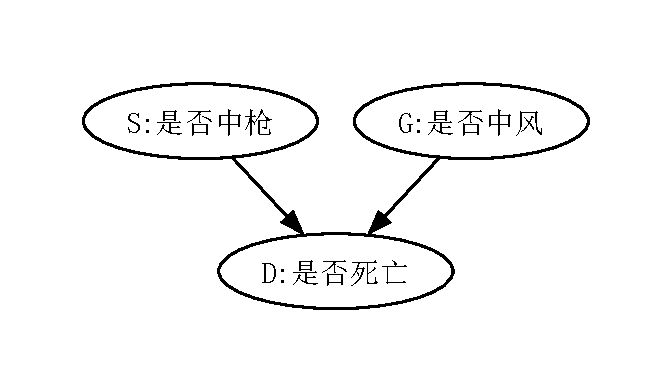
\includegraphics[width=0.5\textwidth]{image/对撞路径例子.pdf}}
	\caption{伯克森悖论}
	\label{fig:berkson}
\end{figure}

图\ref{fig:berkson}中展示了一例:众所周知,枪击和中风都会导致生命的消散,但是人的生命只有一次也不能复活,因而如果一定要死(也就是这两种死法),也只能够选择其中一种,显然,被枪打死的人不可能再中风死,在观察时若我们如果只看到死在这两种死法下的个体,则轻易可以得出中枪死与中风死有着负向相关的关系。

\paragraph*{辛普森悖论(Simpson’s Paradox)}是统计学中著名的聚合现象,指数据在整体层面呈现某种趋势,但按某一变量分层后,各子组的趋势方向与整体相反。

\begin{figure}[ht]
	\centering
	\fbox{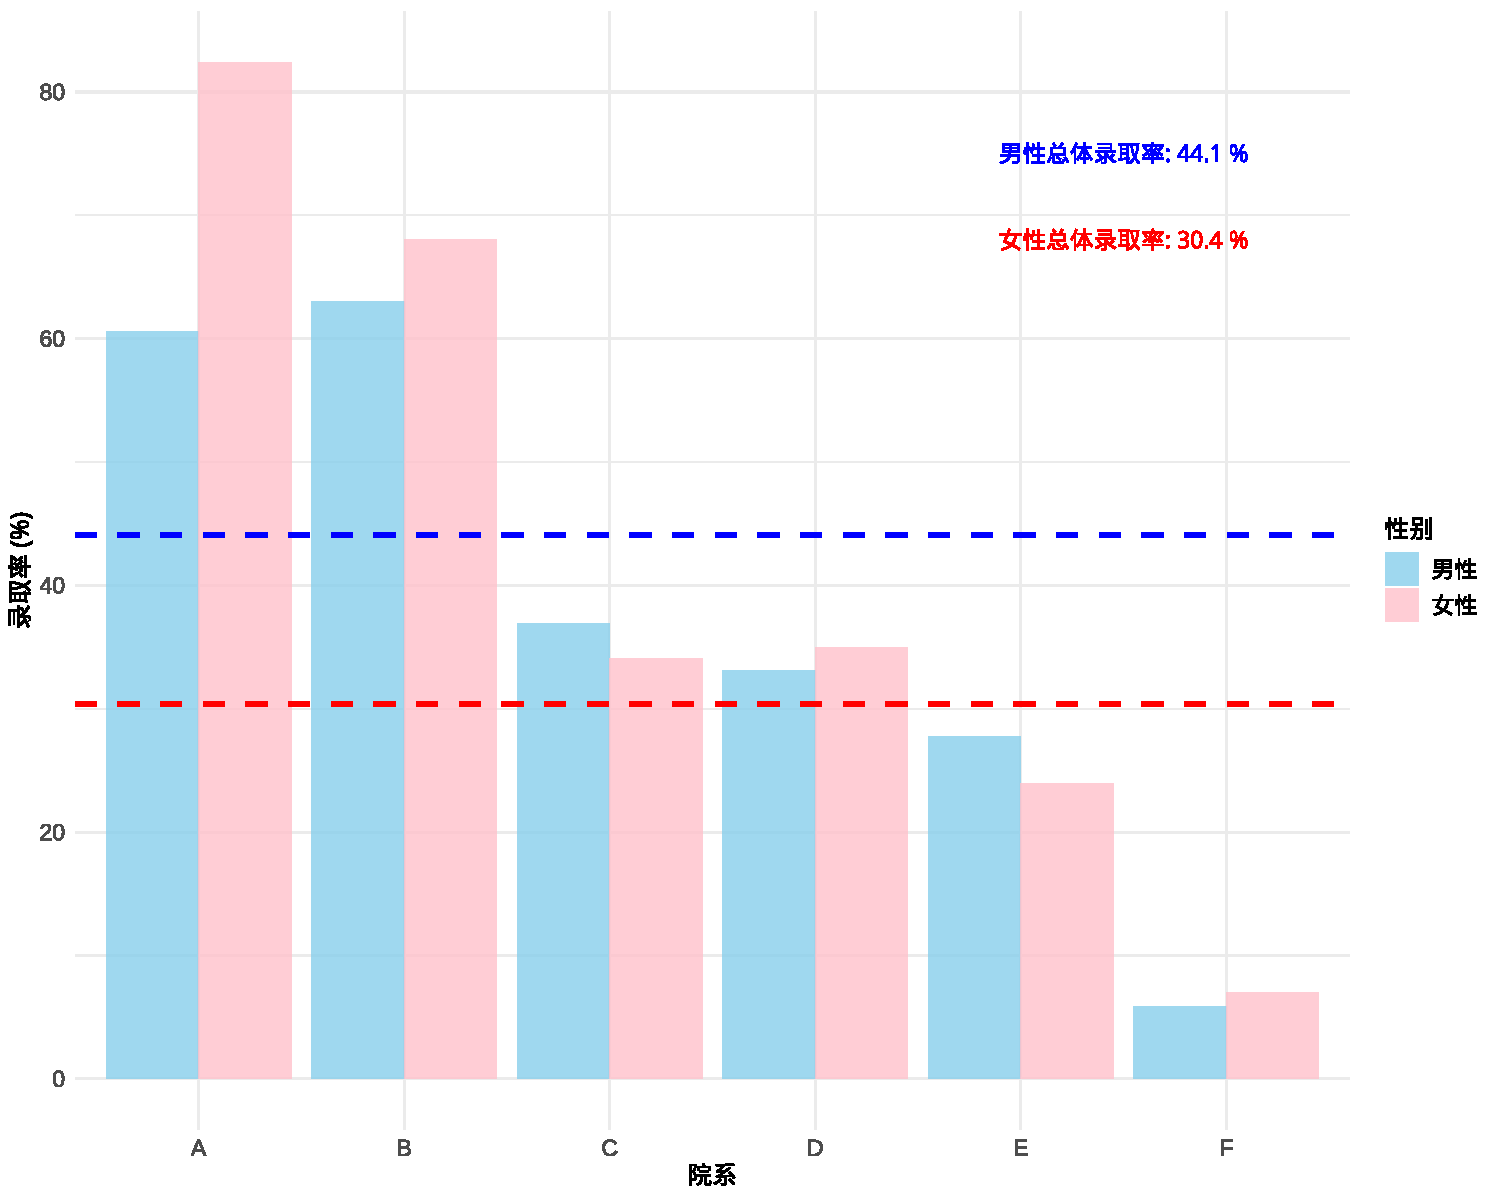
\includegraphics[width=0.5\textwidth]{image/simpson_paradox.pdf}}
	\caption{辛普森悖论}
	\label{fig:simpson}
\end{figure}

典型案例即为伯克利研究生院性别录取率差异,总的来看,男性的录取率高于女性(44.1\%大于30.4\%),但当我们把研究生院再划分为不同的院系后,大部分院系对于女性的录取率实际高于男性(见图\ref{fig:simpson})。彼得·比克尔(Peter Bickel)认为这一现象乃处于女性更倾向于申请竞争压力较大的院系,在这种情况下,大量的陪跑案例当然拉低了总的录取率。该悖论揭示了忽视混杂变量可能导致的错误推论,强调分层分析与因果推断中考虑潜在混杂因素的必要性。

\paragraph*{罗德悖论(Lord’s Paradox)}指同一数据集通过不同统计方法分析可能得出矛盾结论的现象。这一悖论最早由统计学家弗雷德里克·罗德(Frederic Lord)在1967年提出,揭示了数据分析中一个关键问题:统计方法的选择如何影响研究结论,尤其是在涉及协变量调整时。

\begin{figure}[ht]
	\centering
	\fbox{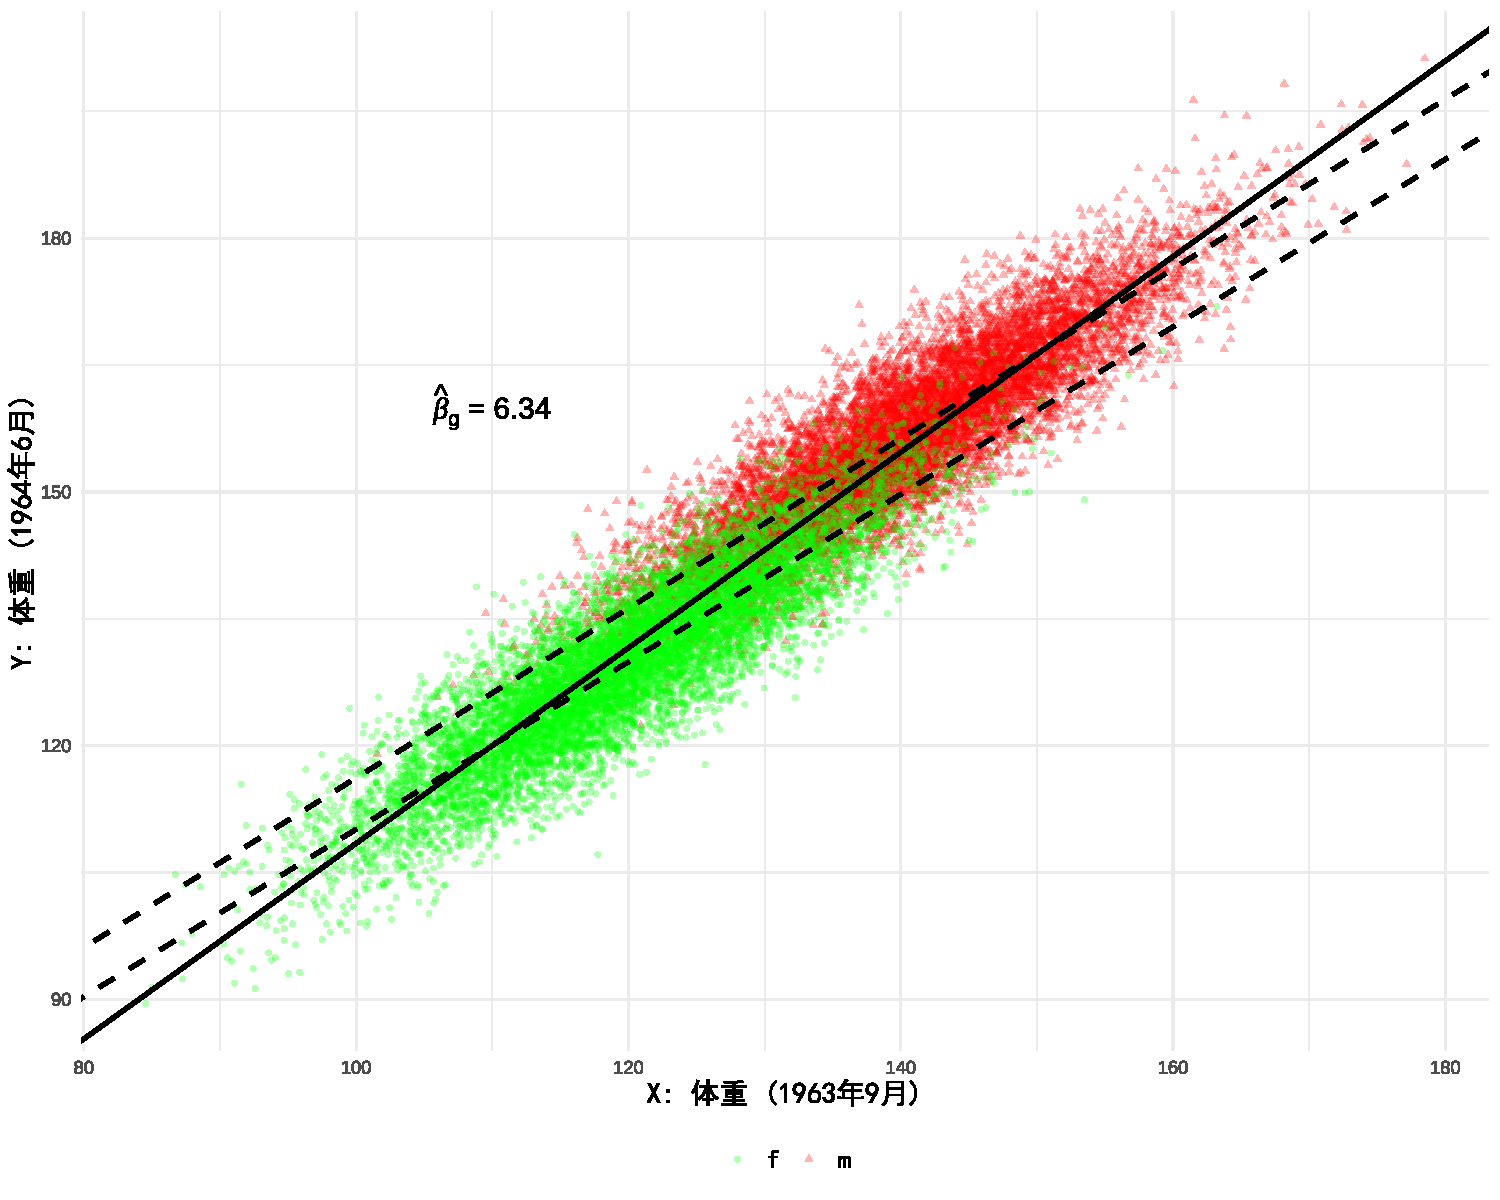
\includegraphics[width=0.5\textwidth]{image/lords_paradox.pdf}}
	\caption{罗德悖论}
	\label{fig:lord}
\end{figure}

在罗德的研究案例中,两位统计学家对同一组数据(学生入学体重X和一年后体重Y,图\ref{fig:lord})进行分析,却得出截然相反的结论:

\begin{enumerate}
	\item 简单均值比较:第一位统计学家直接比较男女学生的体重变化均值,发现两组均无显著变化,因此认为食堂对体重无影响。
	\item 协方差分析(ANCOVA):第二位统计学家学过控制入学体重(X)后,发现男女学生的体重变化存在显著差异(截距差为6.34磅),认为食堂对男女影响不同。
\end{enumerate}

这一矛盾表明,是否调整协变量可能导致研究结论的差异,其背后的根本问题在于,我们无法得知不吃食堂这一反事实(counterfactual)条件下男女的体重情况(没有对照组),因而使得回归或者协方差分析等统计工具失效,并不能清楚地回答有关因果的问题。

通过因果图的形式,我们可以更直观地看到这些悖论的出现,此处可以跳到图\ref{fig:relation}复习。显然,这些变量关系在本章中又再次出现,由于已经引入了因果图的概念,我们可以对其进行案例化,如图\ref{fig:wahaha}:

\begin{figure}[ht]
	\centering
	\fbox{
\includegraphics[width=0.5\textwidth]{image/wahaha.png}}
	\caption{财产分配的因果图}
	\label{fig:wahaha}
\end{figure}

在某企业家引发的舆情事件中,我们尝试提炼出一个关于社会关系继承的因果机制模型。首先,从死亡方式切入,该企业家据称因病去世(例如中风),这一前提将我们讨论的问题限定在“自然死亡”或“疾病死亡”等非暴力性死亡情境之中。这一设定本身即排除了如枪击等“非自然死亡”情境所涉及的诸多干扰因素,从而有助于厘清自然死亡背景下的社会关系变动,当然我们在做大样本分析时不能排除非自然死亡的情况。

然而,在因果分析中一旦引入“是否死亡”作为控制变量,便可能无意间触发“\textbf{对撞偏差}”(collider bias)的问题:当一个变量(如“是否死亡”)同时受到两个原本无关联的因素(如“是否中风”与“是否枪击”)影响,且被纳入分析模型时,会在它们之间引入人为关联,从而扭曲对因果路径的识别。例如,死亡作为既成事实,是我们观察遗产分配问题的前提,而死亡方式作为路径条件,本应是划定分析边界的工具。但当我们将“是否死亡”作为控制变量时,原本独立的“是否中风”与“是否枪击”两个变量便在图式中联通,形成类似“ $ \text{是否中风} \rightarrow \text{是否枪击} \rightarrow \text{确立遗嘱}$ ”这样的虚假因果路径。这种结构性错误会削弱我们对“自然死亡背景下遗嘱确立行为”这一主路径的识别能力。

进一步而言,“确立遗嘱”通常通过影响“家庭关系”间接作用于“财产分配”,家庭关系因而可被视作一个具有机制意义的中介变量。该路径结构揭示出财产继承不仅是个人意愿的体现,也是亲属关系结构的延续与反映。然而,若研究者试图将所有可能的中介路径一并纳入模型进行调整(例如控制家庭互动频率、情感亲疏、文化观念等),则可能落入“\textbf{过度控制偏差}”(over-control bias)的陷阱。在这种情况下,“个人意愿”这一关键变量的真实效应,可能被其他解释变量的残差结构所吸收,从而妨碍我们对主因路径的识别与估计。

在死因探讨之外,“日常为人”(例如企业家的性格、道德声誉、人际互动方式等)不仅可能影响其家庭关系,也可能对其财产分配产生前因上的作用。因此,“日常为人”作为一个潜在混淆变量,若未被纳入分析,将可能引发如“辛普森悖论”这类由于聚合数据忽视分层关系而造成的推断错误,也叫“\textbf{混淆偏差}”(confusion bias)。

此外,不容忽视的是“法律制度”等宏观背景变量。虽然其通常具有高度稳定性,短期内不易观察其变化,但在长时段演化中,其对遗嘱制度与财产分配的规范作用不可忽略。尽管制度或文化等外在环境因子的量化困难重重,但已有研究通过创新方法成功应对这一挑战。

\subsection{截断}

面对上述的复杂因果关系,我们似乎难以把握,尤其是如何精准地提取出X对Y的影响。事实上,指望在统计学范畴内予以彻底解决——尤其是在社会科学领域中试图收集关于全体变量的完备数据——几乎是不可能的任务。正因如此,珀尔提出了“干预主义”思想,并以do算子为工具,试图跳出被动观察的框架,主动设定变量的状态,从而厘清因果路径。

然而,即便引入了干预操作,我们仍需回答一个基础性问题:在干预变量X的同时,是否还有其他路径会影响到Y?亦即,我们如何“截断”所有除 $X \rightarrow Y$ 之外的混杂路径,只保留真正的因果链?为此,理解路径结构是至关重要的,以下两类共四种路径类型构成了因果图分析的基础。

\paragraph*{前门路径}

前门路径指的是一种通过中介变量传导的路径,即存在一条 $X \rightarrow M \rightarrow Y$ 的路径,其中M是介于X与Y之间的中介变量。若前门路径独立于所有混杂路径,并且X对M与M对Y的因果关系均可识别,那么通过控制M这一中介变量,即可在未观测混杂变量Z的前提下识别 $X \rightarrow Y$ 的因果效应。这便是所谓“前门准则”(front-door criterion)所依赖的结构条件。

在上述的例子当中,当我们认定生前为人对家庭关系并无影响的情况下,便可以通过估测是否死亡对家庭关系( $X \rightarrow M$ )以及家庭关系对遗产分配( $M \rightarrow Y$ )得出一个确立遗嘱对遗产分配( $X \rightarrow Y$ )的因果效应来。

前门路径的核心优势在于:它不要求我们观测并控制所有影响 $X$ 和 $Y$ 的共同原因,而是通过中介变量的“结构绕行”实现了因果推断。这也体现出结构因果模型(SCM)在非实验数据中的强大推理能力。

引入do算子之后,我们关注的已不再是观察性条件概率 $P(Y \mid X)$,而是介入性概率 $P(Y \mid do(X))$。这是因为 $do(X)$ 表示我们人为地设定变量 $X$ 的值,从而切断 $X$ 与其上游变量(包括潜在混杂变量 $Z$)之间的自然因果联系。这一操作是实现因果推断的关键步骤。

在满足前门准则的前提下,$P(Y \mid do(X))$ 可以通过如下公式进行识别:

\begin{equation}
P(Y \mid do(X)) = \sum_{m} P(M = m \mid X) \sum_{x'} P(Y \mid M = m, X = x') P(X = x')
\end{equation}

这一表达式背后的逻辑如下:我们首先利用 $P(M \mid X)$ 捕捉 $X$ 对中介变量 $M$ 的因果影响,然后通过对所有可能的 $x'$ 求和来消除 $X$ 与 $M$ 之间的关联性,进而评估 $M$ 对 $Y$ 的因果影响。由于 $M$ 同时受到 $X$ 的影响并影响 $Y$,其在传导因果效应的过程中起到了桥梁作用。

继续回到前述的社会情境例子,在认为“为人”不影响“家庭关系”的前提下,如果我们能观测并建模“是否立遗嘱”对“家庭关系”的影响($X \rightarrow M$),以及“家庭关系”对“遗产分配”的影响($M \rightarrow Y$),则即便存在无法观测的混杂变量(例如家族文化、遗产规模、潜在冲突历史等),但由于这些混杂变量不直接影响到家庭关系这一中介变量,故我们仍可以通过前门准则识别 $X$ 对 $Y$ 的净因果效应,如图\ref{fig:wahaha2}所示。

\begin{figure}[ht]
	\centering
	\fbox{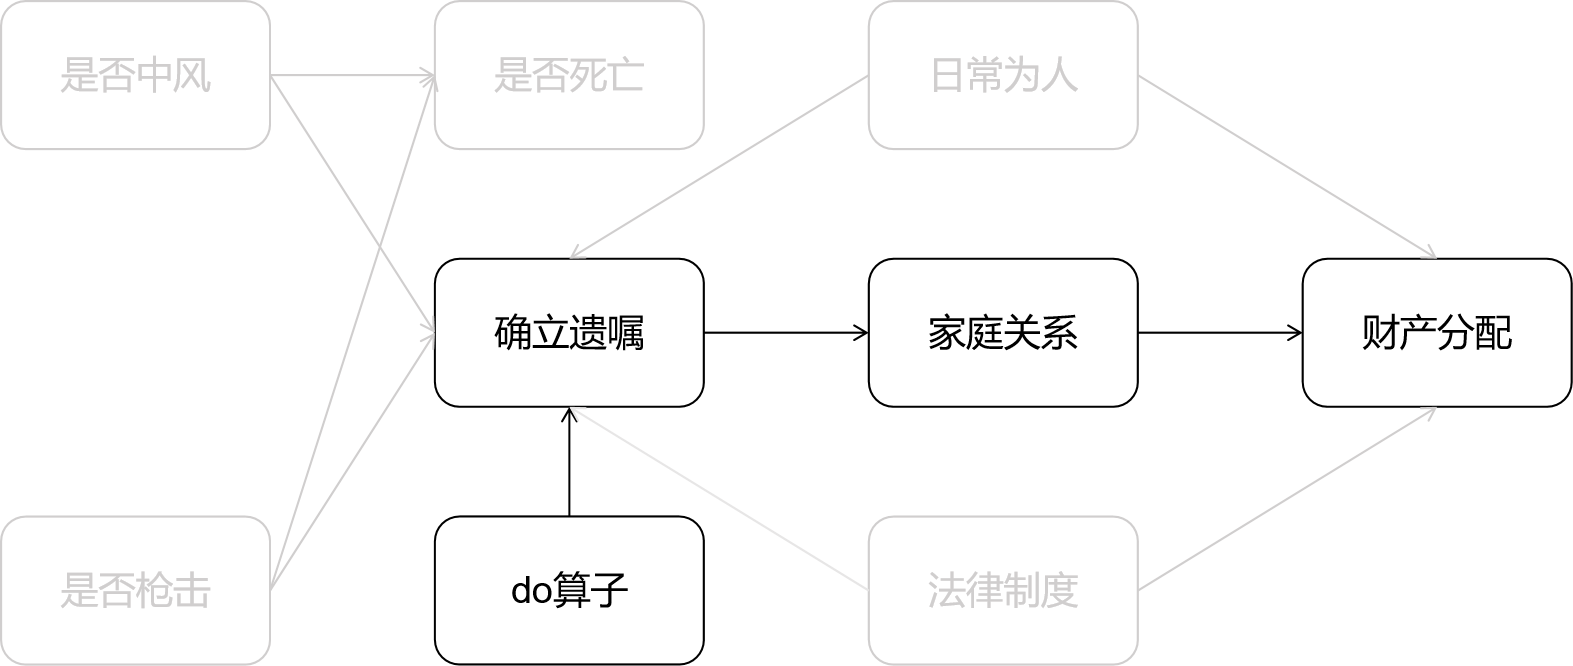
\includegraphics[width=0.5\textwidth]{image/wahaha2.png}}
	\caption{前门路径示例图}
	\label{fig:wahaha2}
\end{figure}

\paragraph*{后门路径}

相比之下,后门路径是一条从 $X$ 开始,并通过其他变量“绕道”影响 $Y$ 的路径,但其首个箭头是指向 $X$ 的,例如 $X \leftarrow Z \rightarrow Y$。这样的路径通常并不代表真正的因果传导链条,而是一条混杂路径(confounding path),会引入 $X$ 与 $Y$ 之间的虚假相关性,从而干扰我们对 $X \rightarrow Y$ 因果效应的识别。

为了封闭此类路径,我们需要控制这些共同前因(common causes),即将变量 $Z$ 纳入模型作为控制变量,使得在条件化 $Z$ 之后,$X$ 与 $Y$ 之间的关联可以被解释为因果效应。如图\ref{fig:wahaha3} 示,在我们的实际社会例子中,“日常为人”与“法律制度”可能既影响立遗嘱的行为,也影响财产分配的结果,因此构成混杂变量,需予以控制。

珀尔提出的“后门准则”(back-door criterion)是识别这类因果效应的重要工具。具体而言,若存在一个变量集合 $\mathbf{Z}$ 满足:

\begin{itemize}
	\item 所有从 $X$ 到 $Y$ 的后门路径都被 $\mathbf{Z}$ 所阻断;
	\item $\mathbf{Z}$ 不包含任何 $X$ 的后果(即不包括 $X$ 的子节点,否则变为内生性问题)。
\end{itemize}

则因果效应 $P(Y \mid do(X))$ 可通过如下方式识别:

\begin{equation}
P(Y \mid do(X)) = \sum_{z} P(Y \mid X, Z = z) P(Z = z)
\end{equation}

在该表达式中,$P(Y \mid X, Z)$ 是在观测数据中可以直接估计的条件概率,而 $P(Z)$ 是混杂变量的边际分布。通过对所有 $z$ 的加总,我们相当于模拟了一个“随机赋值” $X$ 的实验情境,从而排除了由于 $Z$ 引起的混杂偏误。

需要特别强调的是,这一公式的左侧为 $P(Y \mid \mathbf{do}(X))$,表示我们关心的是在人为地干预 $X$ 为某一特定值时,$Y$ 的响应分布——这是因果推断的核心目标。右侧虽然只涉及观察性概率(即没有 $do$),但由于我们通过控制混杂变量 $Z$ 封闭了所有非因果路径,进而使得 $P(Y \mid X, Z)$ 可以作为 $X \rightarrow Y$ 因果效应的替代估计。

换言之,这一加权求和过程相当于在每个 $Z=z$ 的条件下估计 $X$ 对 $Y$ 的局部因果效应,并按 $Z$ 的边际分布 $P(Z)$ 进行整合,从而还原出全局的干预效应 $P(Y \mid \mathbf{do}(X))$。通过这种方式,我们实现了从观察性数据中“模拟实验”,使得不具备随机化条件的数据也能够进行有效的因果识别。

后门准则的实质是:在能够观测并控制混杂变量的前提下,我们可以通过调整(adjustment)还原出一个近似实验的因果估计。而do算子的引入则使得这种估计从统计相关性上升为因果推断。


\begin{figure}[ht]
	\centering
	\fbox{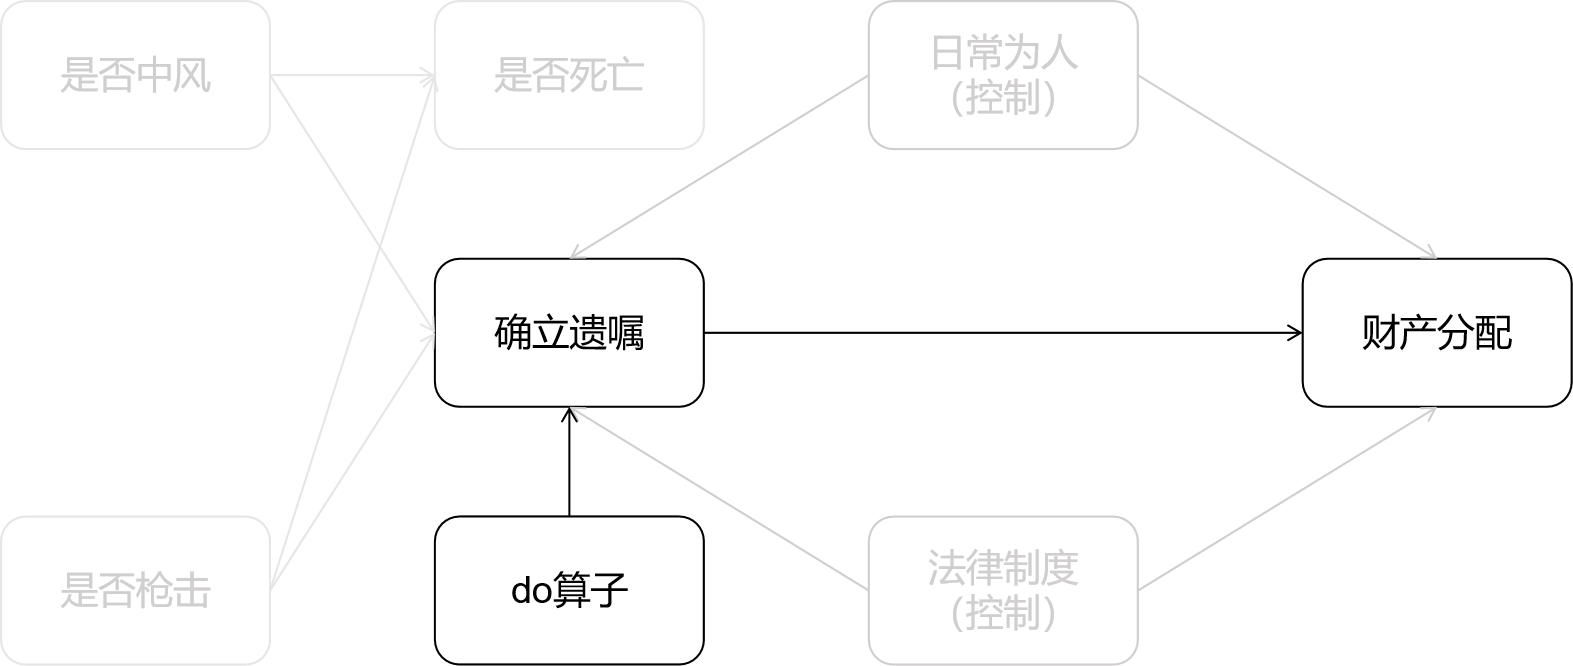
\includegraphics[width=0.5\textwidth]{image/wahaha3.png}}
	\caption{后门路径示例图}
	\label{fig:wahaha3}
\end{figure}

\paragraph*{开路径}

所谓“开路径”是指一条变量之间的路径,其结构在没有被控制的前提下,允许信息在变量间流通,从而导致相关性。在因果图中,如果路径中的所有非冲节点(collider)未被控制,且没有冲节点的后代被控制,那么这条路径就是“开”的(也就是因果图中因能走向果)。这意味着X与Y之间可能因该路径而存在关联,尽管这种关联未必具有因果含义。因此,在识别因果关系时,必须将所有不希望开启的路径加以“\textbf{截断}”。

\paragraph*{死路径}

与“开路径”相对,死路径指的是在控制某些变量后,使路径上出现冲节点或其后代,从而阻断信息流通的一条路径。典型的死路径形式是当路径中存在冲节点(如 $X \rightarrow W \leftarrow Y$)且未控制W或其后代时,该路径自动封闭,变量之间不再相关。对撞路径实际上便是一条死路经,显然,“是否中枪”与“是否中风”的关联完全是由于死亡这一结果而出现,两者间实际上并无瓜葛。这一特性在因果识别中尤为关键,因为它说明并非所有路径都需要控制,有些路径由于结构上的封闭性天然为“死路径”,不构成混杂来源,控制其反而造成“对撞偏差”。

尽管珀尔的理论如此完备,想要据此寻找可行的前门路径和截断所有后门路径仍然不太可能,结构式的复杂也在此凸显无疑,当下的计量经济学似乎是,也仍然将是简约式的主场,通过设计,我们实现了在找不齐路径中变量的情况下仍然能控制偏差的壮举。

\subsection{设计}

现代因果推断的思想萌芽可以追溯到19世纪,但其形式化理论的奠基主要发生在20世纪。回顾林德医生的实验,其核心逻辑——通过人为控制变量,比较处理与非处理之间的差异——与现代实验设计高度一致。这种逻辑,正是后世“潜在结果框架”(Potential Outcomes Framework)所要精确表达的内容。

这一框架的发展历经了数位巨擘的奠基。因此,它通常被称为“奈曼—鲁宾因果模型”(Neyman-Rubin Causal Model, RCM)。其发展脉络清晰地体现了理论的演进:

\begin{itemize}
    \item 耶日·奈曼 (Jerzy Neyman, 1923) 在其关于农田实验的研究中,首次引入了“潜在结果”的数学符号,用以定义不同处理下的潜在产量。这为因果效应的量化提供了数学语言,但当时仅限于随机化的实验场景。
    \item 罗纳德·费舍尔 (Ronald Fisher, 1925) 提出了将处理“随机化”分配给单元是进行因果推断的“合理基础”。他强调了物理随机化在创造可比组别、消除系统性偏差方面的核心作用,使随机对照实验(RCT)成为因果推断的“黄金标准”。
    \item 唐纳德·鲁宾 (Donald Rubin, 1974) 将潜在结果框架从纯粹的实验环境推广至观察性研究,使其成为一个普适的因果分析工具。他明确指出,无论数据来源如何,因果效应的核心定义都应基于潜在结果的比较,并正式提出了“分配机制”在因果识别中的重要性。
\end{itemize}

\paragraph*{核心概念}

鲁宾因果模型的核心构件包括三个基本概念:干预 (Treatment)、潜在结果 (Potential Outcome)与干预效应 (Treatment Effect)。

\begin{itemize}
    \item \textbf{干预}:指研究中所施加的某种处理或变化,通常是我们试图识别其因果影响的自变量。
    \item \textbf{潜在结果}:指在不同干预状态下,一个研究对象可能产生的因变量取值。例如,$Y_i^1$ 表示单位 $i$ 接受处理后的结果,$Y_i^0$ 表示其未接受处理(处于对照状态)的结果。
    \item \textbf{干预效应}:即同一单位在两种状态下潜在结果的差值,是我们最终希望估计的因果量。
\end{itemize}

该框架揭示了被霍兰德(Paul Holland)称为的所谓的“因果推断的根本问题”(Fundamental Problem of Causal Inference, FPCI):对于任一研究对象,在特定时间内只能处于一种处理状态,因此我们永远只能观察到一个潜在结果,另一个则永远处于未被观察到的反事实状态。这种结构性的“数据缺失”是因果分析的核心挑战。

\paragraph*{估计目标}

根据作用层级的不同,干预效应可分为个体层面与总体层面。

\begin{itemize}
    \item 个体干预效应 (ITE, Individual Treatment Effect)指单位 $i$ 在接受干预与未接受干预状态下结果之差。由于FPCI,该值无法直接观测。
    \begin{equation}
        \delta_i = Y_i^{1} - Y_i^{0}
    \end{equation}
    \item 平均处理效应 (ATE, Average Treatment Effect)是最常用的总体参数,定义为所有个体效应的期望值。
    \begin{equation}
        \delta_{ATE} = E[Y_i^1 - Y_i^0]
    \end{equation}
    \item 处理组的平均处理效应 (ATT, Average Treatment Effect on the Treated)关注处理对实际接受者的平均影响。
    \begin{equation}
        \delta_{ATT} = E[Y_i^1 \mid D_i = 1] - E[Y_i^0 \mid D_i = 1]
    \end{equation}
    \item 控制组的平均处理效应 (ATU, Average Treatment Effect on the Untreated)关注处理对未接受者的潜在平均影响。
    \begin{equation}
        \delta_{ATU} = E[Y_i^1 \mid D_i = 0] - E[Y_i^0 \mid D_i = 0]
    \end{equation}
\end{itemize}

其中,$D_i=1$ 表示个体 $i$ 接受处理,$D_i=0$ 表示未接受处理。

\paragraph*{核心假设}
为了克服 FPCI 并从观测数据中估计因果效应,我们需要依赖一系列关键假设。

\begin{enumerate}
    \item \textbf{稳定单元处理值假设 (SUTVA, Stable Unit Treatment Value Assumption)}:此假设包含两个方面:
    \begin{itemize}
        \item 无干扰,即一个个体的处理状态不会影响其他个体的潜在结果;
        \item 处理无多重版本,即处理的实现方式对所有接受者都是一致的。
    \end{itemize}
    \item \textbf{可忽略性/非混淆性假设 (Ignorability / Unconfoundedness Assumption)}:这是连接潜在结果与观测数据的桥梁。它要求处理的分配独立于潜在结果,在给定一组协变量 $X$ 的条件下。形式化表示为:$(Y_i^1, Y_i^0) \perp D_i \mid X_i$。在随机实验中,由于物理随机化,该假设自然成立(无需条件化)。在观察性研究中,研究者必须通过控制所有相关的混淆变量来尽可能满足此假设。
\end{enumerate}

当这些假设满足时,我们就可以用控制组的观测结果来估计处理组的反事实结果,从而识别因果效应。例如,在满足可忽略性假设时,$E[Y_i^0 \mid D_i = 1] = E[Y_i^0 \mid D_i = 0]$,ATT的估计就成为可能。

\paragraph*{实验设计}
在理想情境下,随机对照实验(RCT)因其能够满足非混淆性假设而被视为“黄金标准”。然而,在社会科学中,由于伦理、成本或操作复杂性,严格的RCT往往难以实施。因此,研究者发展了多种实验设计样式以应对复杂现实。

\begin{itemize}
    \item \textbf{被试间设计 (Between-Subject Design)}:将被试随机分配至互斥的处理组与对照组。这是最经典的设计,其变体包括:
    \begin{itemize}
        \item 前测—后测控制组设计:比较处理前后的变化,控制时间趋势。
        \item 仅后测设计:适用于无法或不宜实施前测的场景。
        \item 所罗门四组设计:综合前两者,用以评估并控制前测本身带来的效应。
    \end{itemize}
    \item \textbf{被试内设计 (Within-Subject Design)}:每个受试者依次接受所有处理条件。该设计能完美控制个体间异质性,但需警惕顺序效应(如学习、疲劳效应)。
\end{itemize}

无论何种设计,其首要目标都在于提升\textbf{内部效度},即确保观测到的因果关系确实来自处理本身。然而,过于理想化的实验可能脱离现实,损害结论的\textbf{外部效度}(泛化能力)。因此,如实地实验 (Field Experiment)等设计,试图在自然情境中施加干预,以求在内部效度与外部效度之间取得平衡。

当严格的实验不可行时,社会科学研究者更多依赖观察性数据,并发展出从自然实验 (Natural Experiments)到准实验 (Quasi-Experiments)等一系列方法,试图在“戴着镣铐跳舞”的条件下,尽可能逼近因果推断的理想状态。

\section{从统计推断到因果推断}

理解因果关系是社会科学的核心任务。传统统计推断在描述相关性方面表现出色,但在揭示因果机制时却面临根本性局限。现代计量经济学试图填补从统计相关到因果推断的鸿沟,其基本目标是在有限的数据约束下,通过形式化建模揭示变量间的因果联系,并对特定政策或干预的效果做出可靠估计。

实践中,计量研究多依赖于观察性数据。其最大特征在于,研究者无法控制处理变量的分配机制,因此极易受到混淆因素的干扰。在这种情形下,内生性成为因果推断最关键的挑战。内生性主要源于三个方面:遗漏变量、测量误差以及互为因果。为了应对这些挑战,计量经济学发展出两大核心分析框架:基于匹配的推断路径与基于回归的推断路径。

\subsection{基于回归的因果推断路径}

回归是社会科学与计量经济学中最为经典的因果推断工具之一。其基本思想是刻画变量之间的条件期望关系,并在此基础上识别出解释变量的因果效应。回归框架的优势在于,它不仅能够通过参数化建模来控制混淆变量,还能够与自然实验或准实验设计相结合,以分离出外生的变动部分。因此,回归分析既是一种描述性方法,也是因果推断的核心工具。

\textbf{线性回归模型}:普通最小二乘法(OLS)是回归分析的起点。其估计建立在零条件均值假设之上,即 $\mathbb{E}[\varepsilon|X]=0$ 这意味着解释变量与误差项不相关。在该假设成立时,OLS估计量不仅无偏一致,而且回归系数可被解释为控制其他变量后,自变量变化对因变量的边际效应。线性回归的灵活性在于,它可以通过加入控制变量来削弱遗漏变量偏误,并通过交互项、非线性变换等方式拓展模型的表达能力。然而,如果零条件均值假设被违反,例如存在遗漏变量、测量误差或反向因果关系,则OLS系数将不再具有因果解释。

\textbf{面板数据模型}:当数据在个体与时间两个维度上同时存在时,面板数据模型成为控制未观测异质性的有力工具。  
\begin{itemize}
    \item \textbf{固定效应模型(FE)}通过引入个体虚拟变量,剥离了所有随时间不变的个体特征,从而避免这些不随时间变化的混淆因素影响估计。
    \item \textbf{随机效应模型(RE)}则假设个体效应是随机的,且与解释变量独立。在该假设成立时,RE能够更高效地利用样本内外的变异。
\end{itemize}

\textbf{工具变量法(IV)}:当解释变量内生时,OLS不再能识别因果效应。此时,工具变量法提供了一个解决方案。一个合格的工具变量必须满足两个条件:

\begin{itemize}
	\item 相关性:工具变量与内生解释变量高度相关;
	\item 外生性:工具变量对结果变量的影响仅通过内生解释变量发挥作用。
\end{itemize}

基于工具变量的\textbf{两阶段最小二乘法(2SLS)}是标准的估计方法。近年来,局部平均处理效应(LATE)的提出进一步澄清了IV估计的识别含义,强调其揭示的是特定人群的“边际个体”效应。

\textbf{准实验设计}:当RCT在实际操作中不可行、成本过高或在伦理上不被允许时,研究者往往会转而利用现实世界中自然发生的“类实验”情境,来识别因果效应。这些方法统称为准实验设计。与RCTs通过研究者主动干预并随机分配处理组和对照组来确保两者在处理前无系统性差异不同,准实验设计则是在非随机分配处理的情况下,通过巧妙的统计方法和识别策略,尽可能地模拟随机化实验的条件,从而从观测数据中抽取出处理变量的因果效应。

\begin{itemize}
    \item \textbf{双重差分法(DID)}专为评估政策或事件冲击而设计,其核心假设是“平行趋势”,即在没有处理的情况下,处理组与对照组应具有相同的时间演化趋势。
    \item \textbf{断点回归设计(RDD)}适用于处理状态由某一连续变量是否超过阈值决定的情境。其关键假设是,在阈值附近个体具有相似特征,因此处理效应可通过阈值两侧的结果差异识别。
    \item \textbf{合成控制法(Synthetic Control)}常用于政策干预的跨区域比较,通过构造一个“合成的对照组”来识别干预效应。
\end{itemize}

\subsection{基于匹配的因果推断路径}

与回归方法不同,匹配方法不依赖于参数化的函数形式假设,而是通过在处理组与对照组之间寻找协变量特征相似的个体进行配对,从而构造一个可比的对立事实。这一方法强调“在可比的个体之间做比较”,以尽可能消除协变量差异带来的选择性偏误。

\textbf{处理效应}:因果推断的核心目标是估计处理效应,即比较同一个体在接受与未接受处理时的结果差异。由于反事实结果不可观测,匹配方法通过寻找“替身”来近似这一比较。常见的处理效应指标包括:平均处理效应(ATE)、处理组的平均处理效应(ATT)、以及条件平均处理效应(CATE)。

\textbf{倾向得分匹配(PSM)}:在高维协变量空间下,直接进行多维匹配非常困难。倾向得分匹配通过估计每个个体接受处理的概率(即倾向得分)来降低维度复杂性。其逻辑为:若在给定倾向得分的条件下,处理分配与结果独立(条件可忽略性假设),则匹配基于倾向得分即可实现因果识别。常见方法包括最近邻匹配、卡钳匹配和核匹配等。

\textbf{匹配的优势与局限}:匹配方法的优势在于其非参数性质,不依赖于线性或特定函数形式的假设,且结果直观易于解释。然而,它也存在明显局限:  
\begin{itemize}
    \item 匹配仅能控制基于可观测变量的选择偏误,无法消除不可观测因素的影响;
    \item 匹配质量高度依赖于协变量的丰富性与重叠性,若缺乏共同支持区间,结果可能偏误;
    \item 在样本有限的情况下,匹配可能带来效率损失。
\end{itemize}

总体而言,回归与匹配代表了现代因果推断中的两类互补路径。回归通过建模来控制混淆因素,并结合准实验设计处理内生性问题;匹配则通过数据预处理直接构造可比组,强调非参数和直观性。在实证研究中,二者常常结合使用:研究者可先通过匹配消除处理组与对照组在协变量分布上的差异,再利用回归模型进行进一步调整,从而获得更为稳健和可靠的因果推断结果。这种“多工具并用”的思路,已成为现代因果推断实践中的常态。

后文将对每一段进行细致地展开,并配有Stata代码案例,基本格式如下:

\begin{tcolorbox}[title=Stata 示例, colback=white, colframe=black, colbacktitle=white, coltitle=black,fonttitle=\bfseries]
 * Stata 输入
	\begin{lstlisting}[xleftmargin=2em]
	quietly sysuse auto, clear // 加载系统自带数据集
	summarize // 描述性统计
	graph bar weight price, over(foreign) // 绘制分组条形图
	\end{lstlisting}
 * Stata 输出
	\vspace{-2em}
	\begin{Verbatim}[commandchars=\\\{\},xleftmargin=2em]

		
    Variable |        Obs        Mean    Std. dev.       Min        Max
-------------+---------------------------------------------------------
        make |          0
       price |         74    6165.257    2949.496       3291      15906
         mpg |         74     21.2973    5.785503         12         41
       rep78 |         69    3.405797    .9899323          1          5
    headroom |         74    2.993243    .8459948        1.5          5
-------------+---------------------------------------------------------
       trunk |         74    13.75676    4.277404          5         23
      weight |         74    3019.459    777.1936       1760       4840
      length |         74    187.9324    22.26634        142        233
        turn |         74    39.64865    4.399354         31         51
displacement |         74    197.2973    91.83722         79        425
-------------+---------------------------------------------------------
  gear_ratio |         74    3.014865    .4562871       2.19       3.89
     foreign |         74    .2972973    .4601885          0          1
	\end{Verbatim}

	\begin{center}
	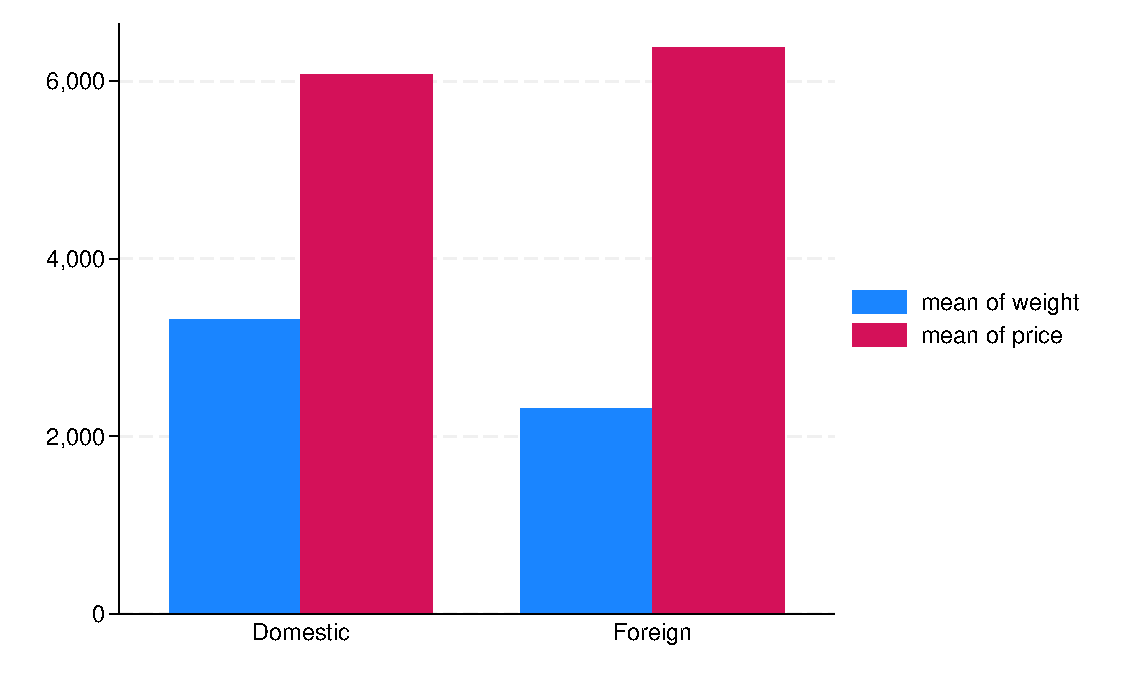
\includegraphics[width=0.8\textwidth]{image/autobar.pdf}
	\end{center}

\end{tcolorbox}

\newpage
\thispagestyle{empty}
\begin{thebibliography}{99}
	\bibitem{1}
	邱嘉平,《因果推断实用计量方法》,上海财经大学出版社

	\bibitem{2}
	赵西亮,《基本有用的计量经济学》,北京大学出版社

	\bibitem{3}
	珀尔 \ 等,《为什么》,中信出版集团

	\bibitem{4}
	安格里斯特 \ 等,《基本无害的计量经济学》,格致出版社

	\bibitem{5}
	游宇 \ 等.一切为了理论——理论化与整合性的案例选择策略[J].世界经济与政治, \\ 2023,(12)

	\bibitem{6}
	许琪.因果推断五十年:成就、挑战与应对[J].学术月刊,2024,56(11)

    \bibitem{7}
	因本斯 \ 等,《因果推断导论》,格致出版社

	\bibitem{8}
	燕继荣 \ 等,《发展政治学学科地图》,北京大学出版社

\end{thebibliography}